\documentclass[conference]{IEEEtran}
\IEEEoverridecommandlockouts
% The preceding line is only needed to identify funding in the first footnote. If that is unneeded, please comment it out.

\usepackage{cite}
\usepackage{amsmath,amssymb,amsfonts}
\usepackage{algorithmic}
\usepackage{graphicx}
\usepackage{textcomp}
\usepackage{xcolor}
\usepackage[pdftex,
pdfauthor={Anjalo Hettiarachchi},
pdftitle={Performance Evaluation of Dynamic Round Robin Algorithms for CPU Scheduling},
pdfsubject={Computer Science},
pdfkeywords={CPU Scheduling,Round Robin (RR),Adaptive Scheduling,Dynamic Time Quantum,Manhattan Distance}]{hyperref}

\newcommand{\BibTeX}{\textrm{B} \kern-.05em{\textsc{i} \kern-.025em b}\kern-.08em T\kern-.1667em\lower.7ex\hbox{E}\kern-.125emX}

\begin{document}

    \title{Performance Evaluation of Dynamic Round Robin Algorithms for CPU Scheduling}

    \author{
        \IEEEauthorblockN{
            Abdulaziz A. Alsulami\textsuperscript{1},
            Qasem Abu Al-Haija\textsuperscript{2},
            Mohammed I. Thanoon\textsuperscript{3},
            Qian Mao\textsuperscript{4}
        }
        \vspace{1em}
        \IEEEauthorblockA{
            Department of Computer Information and Systems Engineering, Tennessee State University,\\
            3500 John A. Merritt Boulevard, Nashville, TN 37209, USA\\
            \\
            \textsuperscript{1}aalsula3@my.tnstate.edu,
            \textsuperscript{2}qabualha@my.tnstate.edu.sa,
            \textsuperscript{3}mthanoon@my.tnstate.edu,
            \textsuperscript{4}qmao@tnstate.edu,
        }
    }

    \maketitle

    \begin{abstract}
        The performance of an operating system (OS) is
        affected by the algorithm policy that is used by a CPU
        to schedule the running processes.~Thus, a better CPU
        scheduling algorithm results in faster OS performance
        using minimal resources over small amounts of time [11].
        For that reason, many algorithms were proposed and implemented
        to enhance the performance of CPU scheduling.~Round Robin is
        considered an efficient and fair algorithm because all
        processes are given the same amount of time quantum.
        However, its efficiency depends on the selected time quantum.
        In this paper, we present a comparative study of four different
        Round Robin algorithms namely: Adaptive Round Robin Algorithm,
        Best Time Quantum Round Robin CPU Scheduling, Optimal Round
        Robin Scheduling Using Manhattan Distance Algorithm, and
        Improved Round Robin Scheduling Algorithm.~We compare these
        algorithms in terms of four performance factors including:
        Average Waiting Time (AWT), Average Turnaround Time (ATT),
        Average Response Time (ART)~and Number of Contexts Switching (NCS).
        The simulation results show that both Adaptive Round Robin
        and Optimal Round Robin Scheduling Using Manhattan Distance
        algorithms are more efficient to be adopted as they recorded
        the minimum values of performance factors.
    \end{abstract}

    \vspace{1em}

    \begin{IEEEkeywords}
        CPU Scheduling, Round Robin (RR), Adaptive Scheduling, Dynamic Time Quantum, Manhattan Distance.
    \end{IEEEkeywords}


    \section{Introduction}
    \label{sec:introduction}
    Due to the significant role of operating systems (OS) in managing
computing resources~\cite{Alsulami2019}~(i.e.~hardware and software
resources)~and providing common services for computer programs, performance
efficiency and ability to manage and schedule several concurrent
processes and tasks is of the utmost importance for a wide range
of applications.~Nowadays, computing platforms are designed with
multiprocessing capabilities and thus equipped with multitasking
operating systems in which a large number of processes can be
scheduled to be executed without users noticing.~Indeed, increasing
the efficiency of CPU scheduling is a challenging issue and thus
several scheduling algorithms were proposed to improve CPU
scheduling and maximize CPU scheduling performance by controlling
and enhancing four different criteria including:

\begin{itemize}
    \item Average Waiting Time (AWT) which is the average time
    that all processes wait in the queue.
    \item Average Turnaround Time (ATT) which refers to the total
    time between the arrival of a process and its completion time.
    \item Average Response Time (ART) which refers to the time
    between the arrival of a process and the time of first
    response to it.
    \item Number of Context Switching (NCS) which refers to the
    number of times that the CPU switches between processes.
\end{itemize}

\begin{figure}[h]
    \centering
    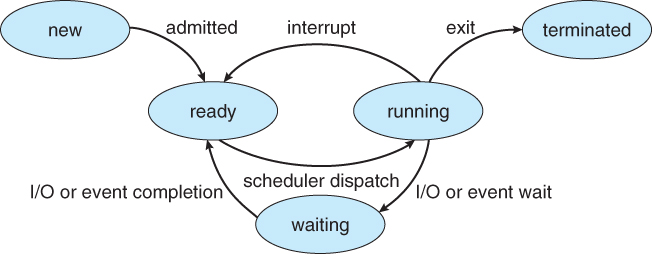
\includegraphics[width=0.45\textwidth]{../figures/figure01}
    \caption{Waiting to Ready CPU Scheduling Scheme [2]}
    \label{fig:fig.waiting-to-ready-cpu-scheduling-scheme-[2]}
\end{figure}

Generally, in order to improve the efficiency of the
CPU, such criteria must be kept to a minimum.~The basic
CPU scheduling scheme is called "waiting to ready" and
illustrated in Figure 1.~In this basic algorithm, if the process
is preemptive, it will not wait any longer to get scheduled.
It will snatch the chance from other lower-priority process.
If the process is having lower priority/non-preemptive, then
it will keep waiting for the resources to release , complete
the event and then get dispatched through the scheduler.
However, a large number of CPU scheduling algorithms that
utilize the aforementioned criteria in their execution were
proposed and analyzed in the literature, for instance:

\begin{itemize}
    \item First Come First Serve~(FCFS): this algorithm executes
    the jobs based on their arrival times, so any process
    that arrives first will be executed.~This algorithm is the
    simplest CPU scheduling algorithm however it produces
    high AWT and ATT.\@
    \item Shortest Job First (SJF): this algorithm executes the jobs
    according to their burst time, so a process with the
    shortest burst time will be executed first.~Hence, this
    algorithm causes starvation of processes that have longer
    burst times.
    \item Round Robin (RR): this algorithm executes jobs with
    specific amounts of time called time quantum.~Therefore,
    all arrival processes will be executed with equal amount
    of time quantum slots.~If a process burst time is greater
    than time quantum it will be blocked and moved to the
    end of the queue and another arrival process will be
    executed.~This algorithm eliminates starvation of processes;
    however, its efficiency depends on selecting the optimal
    value of time quantum.~For example, if the time quantum
    is small, NCS will increase;~however, if the time quantum
    is large, then it will behave as FCFS algorithm [3].
\end{itemize}

\vspace{1em}

There are many researchers developed different solutions
to enhance the performance of RR algorithm, therefore there
is a need to make a comparative study to select the optimal
RR algorithm.~Thus, in this paper, we provide a comparative
study between four different methods that are used to select
optimal time quantum for an RR algorithm that minimizes
the performance criterion factors (i.e., AWT, ATT, ART,
NCS).~The considered RR algorithms include: Adaptive Round
Robin Algorithm [4], Best Time Quantum Round Robin CPU
Scheduling [6], Optimal Round Robin Scheduling Using
Manhattan Distance Algorithm [6], and Improved Round Robin
Scheduling Algorithm [7].~We intentionally chose these four
RR algorithms because their elapsed time are very close to
each other.~Also, we provide extensive simulation results to
evaluate these algorithms according to the aforementioned
factors.\\

The rest of this paper is organized as follows: Section II
presents the related work, Section III describes the Round
Robin Scheduling schemes and its various quantum-based
approaches.~Section IV presents the research methodology and
the simulation results as well as the comparison of the four
algorithms and factors.~Finally, section V concludes the paper


    \section{Related Work}
    \label{sec:related-work}
    In the last decade, several approaches and solutions tried to
    address the efficient utilization of CPU scheduling algorithms
    for processes and jobs (tasks) of the OS. For instance, authors
    of [4] provided a survey study that compared between four
    different algorithms (AAIRR, ERR, AAIRR and ERR).~Each
    algorithm is executed using static and dynamic time quantum.
    Also, there are three cases of generating burst time in case 1
    the burst time was generated randomly, in case 2 burst time
    was generated randomly but in a decreasing order and in case
    3 the burst time was generated randomly but in an ascending
    order.~It is assumed that all processes arrive at the same time
    (arrival time = 0).~The authors use two criteria to examine the
    performance of all four algorithms which is ART and ATT.\\

    Also, in [9] authors compared between two different
    algorithms which are the Improved Round Robin (IRR) which
    has dynamic time quantum, and the basic round-robin which
    has static time quantum.~Selecting the optimal algorithm was
    based on three factors which are AWT, ATT and NCS. The
    experiment has two ceases in case 1 the arrival time is equal
    to 0, and the burst time is generated in an acceding order,
    descending order and random.~In case 2 the arrival time is
    different, and the burst time is generated in an acceding order,
    descending order and random.\\

    There are some limitations in these two researches such
    as in [4] the authors only use two factors in the compression
    between the four algorithms which are AWT and ATT however
    in our research we add two more important factors ART
    and NCS. In [9] Authors compared between two different
    algorithms using three criteria AWT, ATT and NCS however
    the method of generating the burst time, and the arrival time
    was not mentioned.~In our research, we used exponential
    distribution, and the reason of using such a model is explained in
    the next section, Section III, ROUND-ROBIN SCHEDULING
    ALGORITHMS.\@


    \section{Conclusion and Remarks}
    \label{sec:conclusion-and-remarks}
    In conclusion, many Round Robin algorithms were
    developed to maximize the efficiency of the CPU scheduling.
    Therefore, there is a necessity to compare between them by
    evaluating their performance using some criteria such as AWT,
    ATT, ART and NCS. For that reason, this paper compared
    between four different types of RR algorithm.~The simulation
    results showed that both Adaptive Round Robin Algorithm and
    Optimal Round Robin based Manhattan Distance Algorithm
    are more efficient CPU scheduling techniques than Best Time
    Quantum Round Robin CPU Scheduling and Improved Round
    Robin Scheduling Algorithm since they recorded the best
    performance results.

    \bibliographystyle{plain}
    \bibliography{../bib/document}

\end{document}